
\documentclass[10pt,aps, prb,preprint]{article}        
\usepackage{graphicx}
\begin{document}               
\title{Nectar3D: A 3-D Scene Graph Engine in Pure Java\\(First Draft)}
\author{by Lindsay Kay\\lindsay@nectarworks.com}
\date{2 December 2005}
\maketitle

\abstract{
Nectar3D is a simple 3-D scene graph engine in pure Java, featuring shading, depth-cueing and keyframe animation. The Nectar3D renderer fires events when scene elements are picked or moused-over, and may be instructed to highlight selected sets of scene elements. The scene graph can be dynamically modified "at runtime", where elements may be added, deleted or moved while the renderer continually renders it. 
}
\newpage
\tableofcontents
\newpage
\section{Overview}


A Nectar3D scene graph specifies the appearance and behaviour of a 3D world. Elements within a scene can be illuminated with multiple light sources (shaded), made to appear dimmer as they recede into the distance (depth-cued), rendered in order of depth to resolve visual overlap (depth-sorted), and animated through interpolation of their positions, sizes and orientations within keyframe sequences.  The graph can also be partitioned into \textit{layers} which are rendered seperately in the order specified, typically with different rendering features enabled. 
\\
\\
The scene graph is mutable, where elements may be created, destroyed, moved and updated at any time.
\\
\\
A convenient SceneBuilder is provided with which to construct a scene graph, and a SceneRenderer is provided with which to render it. 
\\
\\
Each subtree within a scene can be named so that when an element contained within it is selected from a rendered image (by intersection with given 2-D screen coordinates) the SceneRenderer can fire a selection event identifying the subtree. A set of subtree names can also be specified to the SceneRenderer so that when it renders a scene it will highlight elements within those subtrees. 
\\
\\
The following sections describe the scene graph, SceneBuilder and SceneRenderer.



\newpage
\section{The Scene Graph}
The scene graph is a tree structure over which a SceneRenderer traverses in depth-first, left-to-right order. 
\\
\\
\subsection{Element Types}
The root element of a scene graph is a \texttt{SceneElement}, while all other elements are sub-classes of this type. There are eight types of non-root element:
\begin{itemize}
\item an \texttt{Environment} contains light sources to illuminate sub-elements,
\item a \texttt{Layer} indicates to a \texttt{SceneRenderer} which features it should apply when rendering sub-elements,
\item a \texttt{TransformGroup} specifies transformations to apply to sub-elements,
\item an \texttt{Interpolator} animates a transformation within a parent \texttt{TransformGroup},
\item a \texttt{Geometry} contains \texttt{Point3}s and \texttt{Face}s,
\item a \texttt{Label} is an element of text oriented towards the viewpoint,
\item an \texttt{Appearance} specifies the colour(s) of it's parent, and
\item a \texttt{Name} defines a collective name for sub-elements.
\end{itemize}
These elements are described in more detail in the following sections.


%-------------------------------------------------------
%	Environment
%-------------------------------------------------------


\subsubsection{Environment}
An \texttt{Environment} contains one or more \texttt{LightSource}s, each of which specifies the direction and colour of a light source which illuminates sub-elements. 
\\
\\
Each \texttt{LightSource} has a direction \texttt{Vector3} and a \texttt{Color}. The Nectar3D shading model is Lambertian (flat), where each rendered \texttt{Geometry} \texttt{Face} is uniformly filled by a colour which is a mix of the \texttt{Face}'s original colour and the colours of light reflected from all \texttt{LightSource}s.
\\
\\
Note that the intensity of a \texttt{LightSource} does not attenuate with distance (perhaps this is a feature for the next Nectar3D version).
\\
\\
Although an \texttt{Environment} can be the root of a scene graph, it is typically a child of the root \texttt{SceneElement}, with other \texttt{Enviroments} as siblings. The only type of element that can be a child of a \texttt{Environment} is a \texttt{Layer}. 


%-------------------------------------------------------
%	Layer
%-------------------------------------------------------

\subsubsection{Layer}
A \texttt{Layer} specifies which features should be applied by a SceneRenderer when it renders the \texttt{Layer}'s sub-elements (see Section \ref{SceneRenderer}). 
\\
\\
To see how \texttt{Layer}s work, consider the example scene graph of Figure \ref{fig:layerScene}, which contains objects against a backdrop of sky and ground. This scene has a \texttt{Layer} containing ground and sky as two \texttt{Geometry} sub-elements, perhaps a large green polygon and a large blue polygon. Depth-sorting and shading \textbf{are not} to be applied by a \texttt{SceneRenderer} for that \texttt{Layer}. The second \texttt{Layer} contains an animated \texttt{Geometry} element for a foreground object, and for that \texttt{Layer} those two rendering techniques \textbf{are} to applied by a \texttt{SceneRenderer}. Since a \texttt{SceneRenderer} traverses a scene graph from left to right, the first \texttt{Layer} would be rendered first with the second rendered on top. Note that fogging is not applied to sub-elements of the foreground \texttt{Layer} since fogging blends each element's colours with the scene's background colour (configured with a \texttt{SceneRendererParams} as described in Section \ref{SceneRendererParams}), which is obscurred by the background \texttt{Layer} in this example.

\begin{figure}[!h]
\label{fig:layerScene}
\begin{center}
\scalebox{0.5}{\includegraphics{layerScene.png}}
\caption{UML instance diagram of a scene graph containing background and foreground \texttt{Layer}s. Note how the background layer specifies to a \texttt{SceneRenderer} that it should \textbf{not} apply features such as depthsort and shading when rendering it's sub-elements.}
\end{center}
\end{figure}

The elements that can be direct children of a \texttt{Layer} are:
\begin{itemize}
\item \texttt{Geometry},
\item \texttt{TransformGroup},
\item \texttt{Label},
\item \texttt{Box}, and
\item \texttt{Name}.
\end{itemize}


%-------------------------------------------------------
%	TransformGroup
%-------------------------------------------------------


\subsubsection{TransformGroup}
\label{transformGroup}
A \texttt{TransformGroup} defines a sequence of affine transformations to apply to sub-elements. As described in Sections \ref{geometry} and \ref{label}, the SceneRenderer renders elements such as \texttt{Geometry} and \texttt{Label} after first transforming them by each \texttt{TransformGroup} on the path from the element up to the root.
\\
\\
Affine transformations are added to a \texttt{TransformGroup} one at a time with the element's \texttt{addTransform} method. An element transformed by a \texttt{TransformGroup} is transformed by each of the transformations in the order in which the transformations were added.
\\
\\
 The following constants are defined by \texttt{TransformGroup} to identify the five types of transformations which can be added:
\begin{itemize}
\item \texttt{SCA} - scale on X, Y and Z-axis,
\item \texttt{TRA} - translate on X, Y and Z-axis,
\item \texttt{ROT\_X} - rotate about X-axis,
\item \texttt{ROT\_Y} - rotate about Y-axis, and
\item \texttt{ROT\_Z} - rotate about Z-axis.
\end{itemize}
Each type of transformation can only be added once to a \texttt{TransformGroup}.
\\
\\
Scale factors, translation offsets and rotation angles can be individually set and got for each axis with methods \texttt{setAttribute} and \texttt{getAttribute}. The following constants identify those attributes:
\begin{itemize}
\item \texttt{SCA\_X}, \texttt{SCA\_Y} and \texttt{SCA\_Z} identify factors by which to scale on X, Y and Z-axis,
\item \texttt{TRA\_X}, \texttt{TRA\_Y} and \texttt{TRA\_Z} identify offsets by which to translate on X, Y and Z-axis, and
\item \texttt{ROT\_X}, \texttt{ROT\_Y} and \texttt{ROT\_Z} identify angles in degrees about which to rotate on X,Y and Z-axis.
\end{itemize}

The elements that can be direct children of this element are:
\begin{itemize}
\item \texttt{Geometry},
\item \texttt{TransformGroup},
\item \texttt{Layer},
\item \texttt{Interpolator}, and
\item \texttt{Name}.
\end{itemize}
As described in Section \ref{interpolator}, one or more \texttt{Interpolator}s can be connected as children of a \texttt{TransformGroup} to animate individual transformations.


%-------------------------------------------------------
%	Interpolator
%-------------------------------------------------------


\subsubsection{Interpolator}
\label{interpolator}
An \texttt{Interpolator} animates a single affine transformation within a parent \texttt{TransformGroup}.  An \texttt{Interpolator} contains a series of keyframes, each of which specifies a value for the transformation's attribute at an instant in time, given in milliseconds, relative to the instant that the \texttt{SceneRenderer} was started. 
\\
\\
As described in Section \ref{SceneRendererParams}, a \texttt{SceneRenderer} tracks the milliseconds elapsed since it was started. When a \texttt{SceneRenderer} visits an \texttt{Interpolator}, it updates the \texttt{Interpolator} with the elapsed time. If the \texttt{Interpolator} has two keyframes that enclose the elapsed time it sets the attribute of it's transformation to a value linearly interpolated between the keyframe values as a function of the elapsed time. If no such keyframes exist, the \texttt{Interpolator} does nothing. An \texttt{Interpolator} can therefore be made to lie dormant for a period by specifying a non-zero, positive number of milliseconds for the first keyframe. As long as the elapsed time lies before the first keyframe, the \texttt{Interpolator} lies dormant. When the elapsed time falls after the last keyframe, the \texttt{Interpolator} stops interpolating the attribute. The attribute will remain at the value specified at the last keyframe until some other process modifies it.
\\
\\
TODO: cycling Interpolators!!
\\
\\
An \texttt{Interpolator} can only be a child of a \texttt{TransformGroup} and may not have any child elements.


%-------------------------------------------------------
%	Geometry
%-------------------------------------------------------


\subsubsection{Geometry}
\label{geometry}
A \texttt{Geometry} element contains a list of \texttt{Point3} objects and a list of \texttt{Face}s. Each \texttt{Point3} has double-precision X,Y and Z components, while each \texttt{Face} describes a convex polygon as an array of indices into the \texttt{Point3} list. 
\\
\\
On visiting a \texttt{Geometry} during scene graph traversal a \texttt{SceneRenderer} will first make a copy of it. The \texttt{SceneRenderer} then transforms the copy by each \texttt{TransformGroup} on the path up to the root before rendering it (see Section \ref{transformGroup}). The \texttt{SceneRenderer} does not render \texttt{Face}s which are oriented away from the user (backfaces). Such faces are those for which the angle between the normal vector and the vector towards the viewpoint is greater than 90 degrees, where the normal is computed from the dot product of the first three vertices. 
\\
\\
The only element that can be a child of a \texttt{Geometry} is an \texttt{Appearance} (described in Section \ref{appearance}), to specify to a \texttt{SceneRenderer} the colours to apply to the edges and interiors of the \texttt{Geometry}'s \texttt{Face}'s when rendering or highlighting (see Section \ref{SceneRendererBehaviour}).


%-------------------------------------------------------
%	Label
%-------------------------------------------------------

\subsubsection{Label}
\label{label}
A \texttt{Label} element is a string of text with a \texttt{Font} and an offset on X,Y and Z axis specified by a \texttt{Point3}.
\\
\\
As with a \texttt{Geometry} (see Section \ref{geometry}), a \texttt{SceneRenderer} transforms a copy of each \texttt{Label} by each \texttt{TransformGroup} on the path from the \texttt{Label} up to the root before rendering the copy. Note that the \texttt{Label}'s \texttt{Font} will diminish due to perspective projection.
\\
\\
The only element that can be a child of a \texttt{Label} is an \texttt{Appearance} (described in Section \ref{appearance}), to specify to a \texttt{SceneRenderer} the colours to apply when rendering or highlighting (see Section \ref{SceneRendererBehaviour}).

%-------------------------------------------------------
%	Appearance
%-------------------------------------------------------


\subsubsection{Appearance}
\label{appearance}

An \texttt{Appearance} element specifies to a \texttt{SceneRenderer} colours to apply when rendering the \texttt{Appearance}'s parent element. Four colours are defined by an \texttt{Appearance}:
\begin{itemize}
\item \texttt{fillColor},
\item \texttt{edgeColor},
\item \texttt{highlightFillColor}, and
\item \texttt{highlightEdgeColor}.
\end{itemize}
For a \texttt{Geometry} parent, all four colours specified by \texttt{Appearance} are used to specify fill and edge colours for that parent's \texttt{Face}s  (described in Section\ref{geometry}), as well as alternative fill and edge colours for when highlighting (see Section \ref{SceneRendererBehaviour}).
\\
\\
For a \texttt{Label} parent, only the \texttt{fillColour} and \texttt{highlightFillColour} are employed to specify colours for normal rendering and highlighting of text.
\\
\\
An \texttt{Appearance} can only be a child of a \texttt{Geometry} or a \texttt{Label}, and may not have any child elements.


%-------------------------------------------------------
%	Name
%-------------------------------------------------------


\subsubsection{Name}
A \texttt{Name} element defines a collective name for sub-elements. 
\\
\\
The actual name value of a \texttt{Name} is held in it's \texttt{Selector} property of the \texttt{Name}. A \texttt{Selector} has a \texttt{compare} method which works just like \texttt{java.lang.String}'s method of the same name,  returning -1 if the first is of lower order than the second, 0 if they are equal, or 1 if the second is of lower order than the first.
\\
\\
As described in Section \ref{SceneRendererEvent}, if the mouse is clicked and released over a sub-element of a \texttt{Name}, the \texttt{SceneRenderer} will fire a \texttt{MOUSE\_PICKED} event with a \texttt{Selector} identifying the \texttt{Name}.
\\
\\
To see how \texttt{Name} elements work, consider the example scene graph of Figure \ref{fig:nameExample}. If the mouse is clicked and released over any \texttt{Face} within the two \texttt{Geometry} elements, the \texttt{SceneRenderer} will fire a \texttt{MOUSE\_PICKED} event with a \texttt{Selector} with the value "myHouse".

\begin{figure}[!h]
\label{fig:nameExample}
\begin{center}
\scalebox{0.5}{\includegraphics{nameExample.png}}
\caption{UML instance diagram of a scene graph with a \texttt{Name} element giving the collective name "myHouse" to \texttt{Geometry} elements which model the roof and walls of a house.}
\end{center}
\end{figure}


\subsection{The Scene Graph Builder}
Class \texttt{SceneBuilder} builds a scene graph that is guaranteed to be correctly formed. It is therefore the recommended method by which to build a scene graph from within Java. 
\\
\\
The SceneBuilder works on a metaphor of nested opening and closing of scene elements such that the last element still open is the one to which commands apply. Any command issued that is not relevant to the open element is logged as an error and is otherwise ignored, allowing the build process to continue unaffected. This feature allows more information to be available at once when debugging a long list of building instructions. It can also provides a friendlier user experience when the SceneBuilder is directed by a file parser, where the parser does not neccessarily have to be restarted after each file correction in order to find the next error.
\\
\\
The following code snippet illustrates the use of a \texttt{SceneBuilder}, with indents to clarify nesting:

\begin{verbatim}
SceneBuilder builder = new SceneBuilder();
builder.openEnvironment();
    builder.addLightSource();
    builder.addLightSource();
    builder.openLayer();
        builder.openGeometry();
        builder.close();
    builder.close();
builder.close();
SceneElement scene = builder.buildScene();
\end{verbatim} 


\newpage
\section{The SceneRenderer}
\label{SceneRenderer}
The \texttt{SceneRenderer} is shown in the class diagram of Figure \ref{fig:sceneRenderer}. It is configured with a \texttt{SceneRendererParams} which specifies viewing parameters, and may be given a single \texttt{SceneRendererListener} to handle \texttt{SceneRendererEvents} fired during the rendering process. The following sections briefly describe these last three classes before describing in more detail the behaviour of a \texttt{SceneRenderer}.

\begin{figure}[!h]
\label{fig:sceneRenderer}
\begin{center}
\scalebox{0.4}{\includegraphics{display.png}}
\caption{UML class diagram showing the abstract \texttt{SceneRenderer}, with implementation \texttt{AWTSceneRenderer} which adapts the renderer API to the \texttt{AWT} \texttt{Panel} class and provides double-buffering for flicker-free animation.}
\end{center}
\end{figure}

\subsection{SceneRendererParams}
\label{SceneRendererParams}
Along with viewing parameters a \texttt{SceneRendererParams} also holds the elapsed scene time, which is updated by the \texttt{SceneRenderer} after each frame rendered. A \texttt{SceneRenderer} can be updated with a new \texttt{SceneRendererParams} at rendering time in order to do things such as move the viewpoint, move the projection plane distance for a zooming effect etc.

\subsection{SceneRendererEvent}
\label{SceneRendererEvent}
A \texttt{SceneRendererEvent} has a type identifier and an element of data, the type of which depends upon the type of the event. For \texttt{MOUSE\_PRESSED}, \texttt{MOUSE\_RELEASED}, \texttt{MOUSE\_MOVED} and \texttt{MOUSE\_DRAGGED} the data element will be a \texttt{Point2} indicating the location of the mouse. 
\\
\\
For \texttt{MOUSE\_PICKED} and \texttt{MOUSE\_OVER} events the data will be a \texttt{PickInfo} identifying 
\begin{itemize}
\item a \texttt{Selector} identifying the \texttt{Name} super-element of the nearest element on the Z-axis that intersects the mouse position and
\item the index of the element's primitive (ie. \texttt{Face}) that was clicked on.
\end{itemize}
If the element picked/selected was a cube, for example, the primitive index would indicate which face (0-5) was clicked on. 

\subsection{SceneRenderer Behaviour}
\label{SceneRendererBehaviour}
Figure \ref{fig:rendererStates} shows the three states of a \texttt{SceneRenderer}: \texttt{STATE\_STOPPED}, \texttt{STATE\_RENDERING} and \texttt{STATE\_HIGHLIGHTING}. Initially a \texttt{SceneRenderer} is in \texttt{STATE\_STOPPED}, where it has not yet been given a scene graph to render. 

\begin{figure}[!h]
\label{fig:rendererStates}
\begin{center}
\scalebox{0.4}{\includegraphics{states.png}}
\caption{UML state diagram showing the states of a \texttt{SceneRenderer}}
\end{center}
\end{figure}

\subsubsection{STATE\_STOPPED}
In this state the \texttt{SceneRenderer} awaits a scene graph to render. As soon as it gets one, it transitions to \texttt{STATE\_RENDERING}. If \texttt{SceneRenderer} was not given a \texttt{SceneRenderParams} before it is given the scene graph, it will start \texttt{STATE\_RENDERING} with it's own default \texttt{SceneRenderParams}. 
\\
\\
Any directions to highlight or un-highlight are ignored in this state.

\subsubsection{STATE\_RENDERING} 
In this state the \texttt{SceneRenderer} continually renders it's scene, updating \texttt{Interpolator}s with the time elapsed for each frame. 
\\
\\
If updated with new \texttt{SceneRenderParams} the \texttt{SceneRenderer} will continue \texttt{STATE\_RENDERING}. A \texttt{SceneRenderer} stores the current elapsed time in it's \texttt{RenderParams}, so if the scene \texttt{Interpolators} are to continue where they left off before the update, the new \texttt{RenderParams} should have the same elapsed time value as the last \texttt{RenderParams}. 
\\
\\
If updated with a new scene graph the renderer will continue \texttt{STATE\_RENDERING} the new scene with time continuing to elapse from where it left off.
\\
\\
A highlight direction specifies a list of \texttt{Selector}s corresponding to scene \texttt{Name} elements. When directed to highlight when \texttt{STATE\_RENDERING}, the \texttt{SceneRenderer} will transition to \texttt{STATE\_HIGHLIGHTING}.

\subsubsection{STATE\_HIGHLIGHTING}
In this state \texttt{SceneRenderer} starts by re-renderering it's last image with sub-elements of the specified \texttt{Name}s highlighted. The \texttt{SceneRenderer} will then remain \texttt{STATE\_HIGHLIGHTING}, with time and \texttt{Interpolations} suspended. 
\\
\\
If updated with new \texttt{SceneRenderParams} or a new scene the \texttt{SceneRenderer} will transition back to \texttt{STATE\_RENDERING}. 
\\
\\
If directed to highlight again, the \texttt{SceneRenderer} will again re-renderer it's last image, this time with subelements of the newly selected \texttt{Name} elements highlighted. As before, the \texttt{SceneRenderer} will remain \texttt{STATE\_HIGHLIGHTING}.
\\
\\
Every time a \texttt{SceneRenderer} renders a scene in \texttt{STATE\_RENDERING} it first generates an intermediate 2-D display list of the projections of those polygons which intersect the view volume, which it then renders to the display. Each time the \texttt{SceneRenderer} re-renders the last scene view in \texttt{STATE\_HIGHLIGHTING} it only has to re-draw the 2-D display list, with polygons belonging to highlighted elements rendered in thier highlight colours. 

\subsubsection{Transitions on Error}
Any error that occurs in \texttt{STATE\_RENDERING} or \texttt{STATE\_HIGHLIGHTING} states will cause the \texttt{SceneRenderer} to transition to \texttt{STATE\_STOP}. Errors might be due to running out of memory, divide-by-zero or other conditions that cannot be predicted by scene graph validation.


\newpage
\section{Example of Use}
In this example we will set up a renderer and build a scene graph. We will then render the scene graph with the renderer.
\subsection{Setting up a SceneRenderer}
Let's set up an AWT-compatible \texttt{AWTSceneRenderer} then attach a \texttt{SceneListener} to handle \texttt{SceneRendererEvent}s. This example only handles \texttt{MOUSE\_PICKED} events.
\begin{verbatim}
...

SceneRenderer renderer = new AWTSceneRenderer();

renderer.setListener(
    new SceneListener() {
        public void handleEvent(SceneRendererEvent e) {
            switch (e.getType()) {
                case SceneRendererEvent.ERROR:
                    System.out.println((String)e.getData());
                    break;

                case SceneRendererEvent.MOUSE_DRAGGED:
                    break;

                case SceneRendererEvent.MOUSE_MOVED:
                    break;

                case SceneRendererEvent.MOUSE_OVER:
                    break;

                case SceneRendererEvent.MOUSE_PRESSED:
                    break;

                case SceneRendererEvent.MOUSE_RELEASED:
                    break;

                case SceneRendererEvent.MOUSE_PICKED:
                    PickInfo pickInfo = (PickInfo)e.getData();
                    Selector name = pickInfo.getSelector();
                    System.out.println("Pick event handled: \"" 
                        + name.toString() + "\"");
                    break;
                default:
        }
    }
});
 
SceneRendererParams params = new SceneRendererParams();
params.setFrustum(new Volume3(-200.0, -200.0, -300.0, 200.0, 200.0, -100.0));
params.setWindow(new Window2(0, 0, 800, 800));
params.setVPDist(-500.0);
params.setEye(new Point3(0.0, 0.0, 100.0));
params.setLook(new Point3(0.0, 0.0, 0.0));
params.setUp(new vector3(0.0, 1.0, 0.0));
params.setBackgroundColor(new Color(100, 255, 255)); // Light blue

renderer.setParams(params);

// At this point we would add the renderer to a layout

...

\end{verbatim}
Our renderer is now in the \texttt{STATE\_STOPPED} state and awaits a scene graph. 

\subsection{Building a Scene Graph}
Let's create a scene graph using a \texttt{SceneBuilder}. We'll attach an \texttt{ErrorHandler} to the \texttt{SceneBuilder} to report any errors that occur during the build process, then we'll issue commands to the \texttt{SceneBuilder} to create a scene containing a red cube with yellow edges that rotates 360 degrees over five seconds before stopping. The cube will be illuminated by two light sources, one yellow, the other white. Although probably not noticeable in this example, the cube will fade into a light blue background in proportion to it's depth in the view space (depth cueing). The cube also gets a name, "Hello, World", which our renderer will print to standard output when the cube is clicked on (picked). 

\begin{verbatim}
SceneBuilder builder = new SceneBuilder();

builder.setErrorHandler(new ErrorHandler() {
    public void handleError(String message) {
        System.out.println("Error building scene: " + message);
    }
});

builder.openEnvironment();
builder.addLightSource(new Vector3(1.0,  0.0, 0.0), new Color(60,60,0));
builder.addLightSource(new Vector3(1.0, -1.0, 0.0), new Color(100,100,100));
builder.openLayer("foreground", true, true, true); // Depthsort, depth-cueing and shading
builder.openTransformGroup();
builder.rotateY(0.0);
builder.rotateX(45.0);
builder.openName(new StringSelector("Hello, World!"));
builder.openBox(30.0, 30.0, 30.0);
builder.openMaterial();
builder.setEdgeColor(new Color(255,255,0));        // Yellow
builder.setFillColor(new Color(255,0,0));          // Red
builder.close();
builder.close();
builder.close();
builder.openInterpolator(TransformGroup.ROTY_VAL);
builder.addKeyFrame(0, 0.0); 
builder.addKeyFrame(5000, 360.0);                  // Five seconds
builder.close();                                   // Interpolator
builder.close();                                   // TransformGroup
builder.close();                                   // Layer
builder.close();                                   // Environment

SceneElement  sceneRoot = builder.buildScene();

renderer.setScene(sceneRoot);                      // Rendering starts now
\end{verbatim}

\subsection{Rendering the Scene Graph}


\begin{figure}[!h]
\begin{center}
\scalebox{0.5}{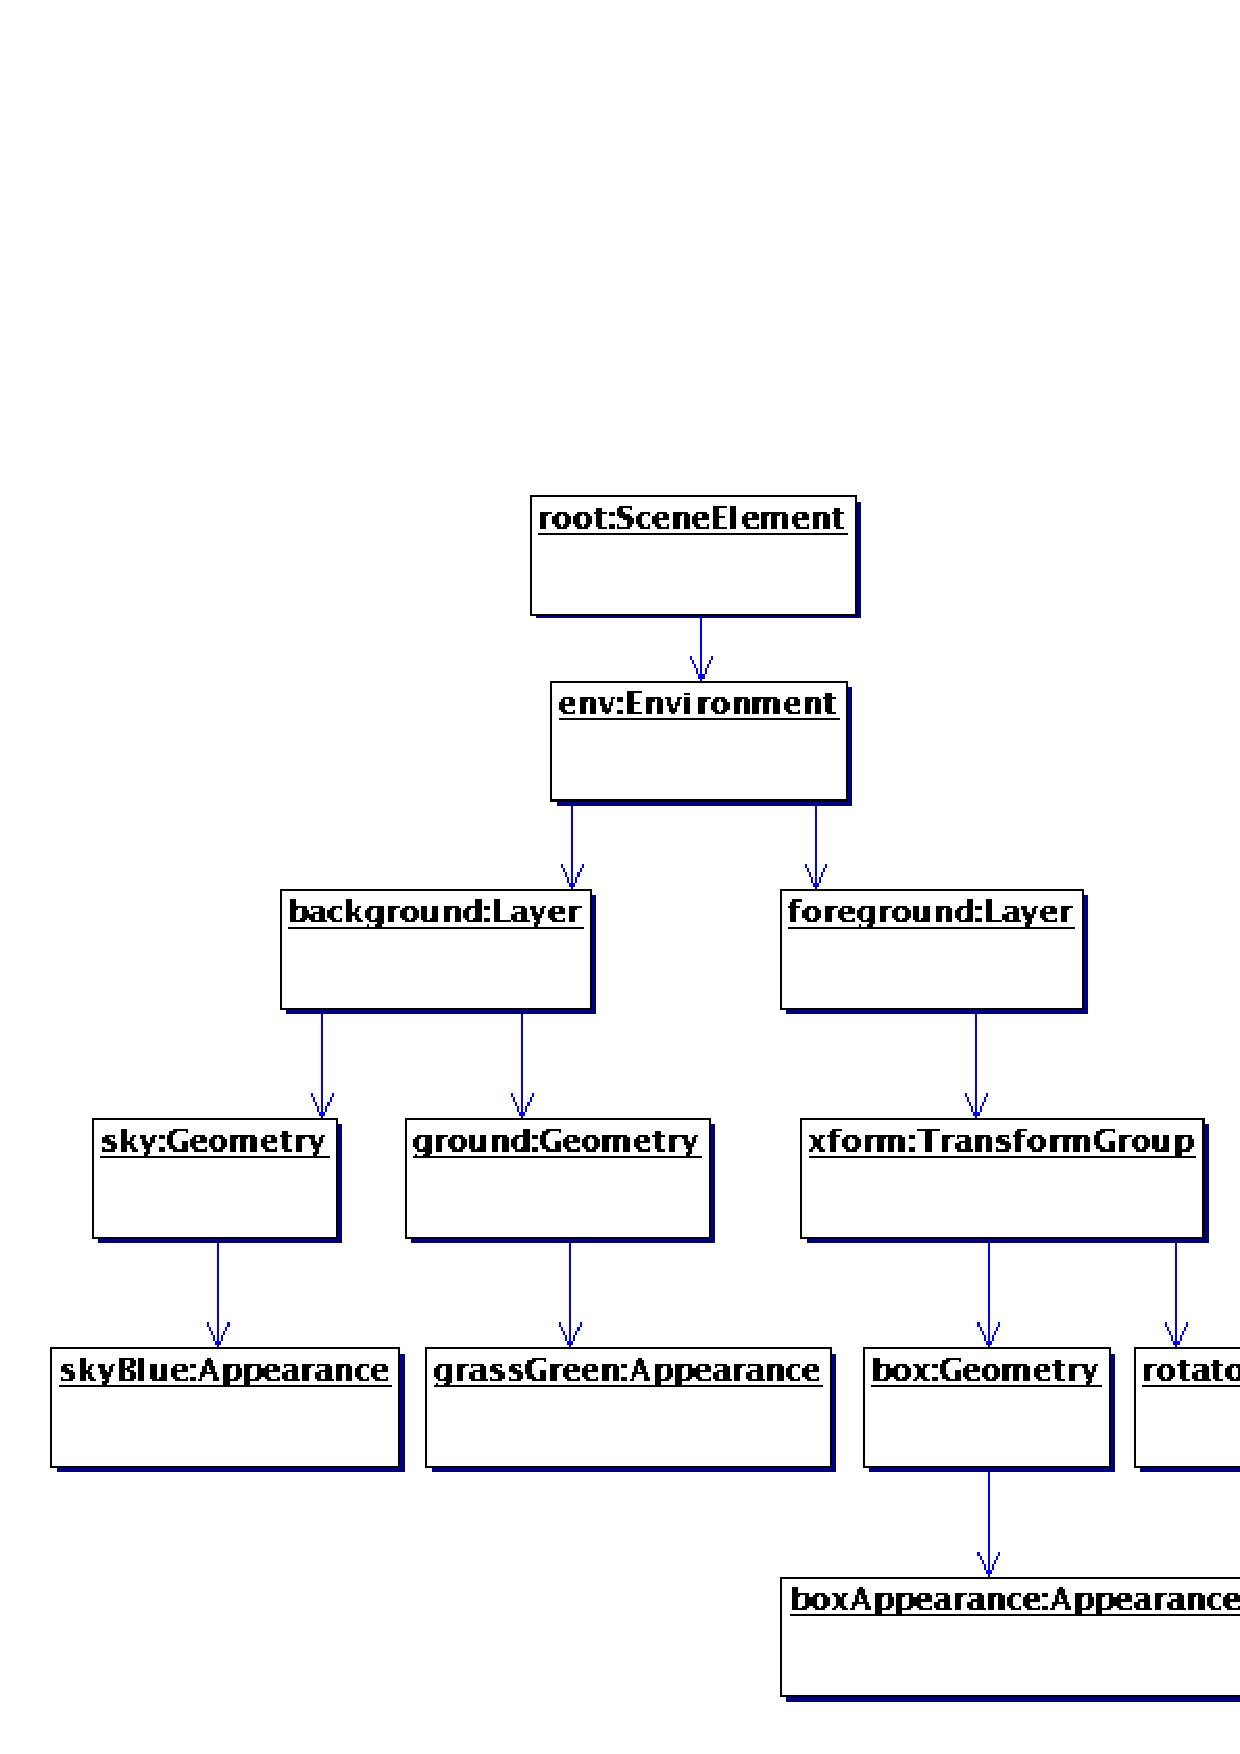
\includegraphics{scene.png}}
\caption{\label{fig:scene}An example scene graph containing a rotating box against backdrop of blue sky and green grass.}
\end{center}
\end{figure}
\newpage
\begin{figure}[!h]
\label{fig:layerScene}
\begin{center}
\scalebox{0.5}{\includegraphics{screenshot1.png}}
\caption{Screen shot}
\end{center}
\end{figure}

\begin{thebibliography}{5}
\bibitem{rife} RIFE Web Application Framework\\ Uwyn\\ www.uwyn.com
\bibitem{echo} Echo Web Application Framework\\ xxx\\ xxx
\bibitem{velocity} Velocity Web Application Framework\\ xxx\\ xxx
\bibitem{swing} Swing GUI Widget Set\\ Sun Microsystems\\ xxx
\bibitem{rifeCont} RIFE Continuations\\ xxx\\ xxx
\end{thebibliography}

\end{document}
